\documentclass[]{article}

\usepackage{graphicx} %for å inkludere grafikk
\usepackage{verbatim} %for å inkludere filer med tegn LaTeX ikke liker
\usepackage{tabularx}
\usepackage{booktabs}
\usepackage{amsmath}
\usepackage{float}
\usepackage{color}
\usepackage{listings}
\usepackage{physics}
\usepackage{hyperref}
\usepackage{subfig}
\usepackage{mhchem}
\usepackage{natbib}
%opening
\title{}
\author{}

\begin{document}
	
\title{Fission: a TALYS report}
\author{Dorthea Gjestvang }
\date{December 2017}

\maketitle

\begin{abstract}
A report based on very crude simulations, concluding that the simulations must be better before they can be reliable
\end{abstract}

\section{Introduction}

In all experimental sciences, one must accept that we only know parameters within a given uncertainty, and experimental nuclear physics is no different. Parameters such as mass, level density and excitation energy are not known as absolute values. This, however, is bothersome when trying to conduct simulations where these values are needed as input. The simulation will be no better than the uncertainty of the values it needs as input parameters. If the simulation additionally is extremely dependent on the values of this imput, the output of the simulation can yield vastly different answers for a slight variation in one of the input variables. It is therefore important to be aware of such dependences when conducting simulations. 

\par 
\vspace{3mm}

In this report, I will first present the theory behind the fission barrier and then what we know about fission's role in the nucleosynthesis. Thereafter, I will test the sensitivity of the (n, $\gamma$) and (n,f) cross sections for $\ce{^{240}Pu}$ upon changes in the fission barrier. Based on this, I can determine whether TALYS might be likely to predict these cross sections correctly before my master experiment runs in April 2018.

\section{Theory}
\label{Theory}
\subsection{Fission barrier}
When observing the average binding energy per nucleon, shown in Figure \ref{fig:binding_energy_per_nucleon}, one can observe that for $A = 56$ the binding energy per A peaks, and then starts to decrease for increasing A. For nuclei situated to the right of this peak, it is thus possible to release energy by splitting in two lighter fragments, that is to fission. However, when studying the chart of nuclei , one will observe that only a handfull of nuclei have spontaneous fission as their main decay mode, and they are generally heavy elements far from the valley of stability. This  is due to the so-called fission barrier. 
\par
\vspace{3mm}

\begin{figure} [tbp]
	\centering
	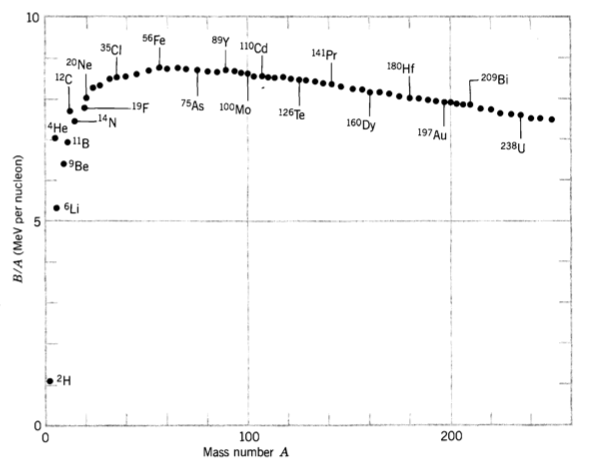
\includegraphics[scale=0.6]{binding_energy_per_nucleon.png}
	\caption{Average binding energy per nucleon. Figure from K.S. Krane p.67 \cite{Krane1988}}
	\label{fig:binding_energy_per_nucleon}
\end{figure}


 \noindent In the liquid model, the fission barrier is described as a smooth, parabolic barrier, and is shown in Figure \ref{fig:smooth_fission_barrier}. It describes the energy needed to separate the two fission fragments as a function of separation distance \cite{Krane1988} [NOTE TO FUTURE DORTHEA: SNAKK MED FABIO OM DENNE (oh hey reader, don't borther with this note)]. The fission barrier is due to both the nuclear force and the Coloumb force. A picture on why there is a fission barrier, is that in order for the two would-be fission fragments to separate, they have to get out of the potential well that is the nuclear force, and then pass the Coloumb barrier. Thus energy must be applied for the fragments to be able to separate. This energy needed is often referred to as the activation energy, and is shown in Figure \ref{fig:smooth_fission_barrier} as the difference in energy between the ground state of the nucleus, and the maximum of the fission barrier potential. 
 
 \par
 \vspace{3mm}
 
 \begin{figure} [tbp]
 	\centering
 	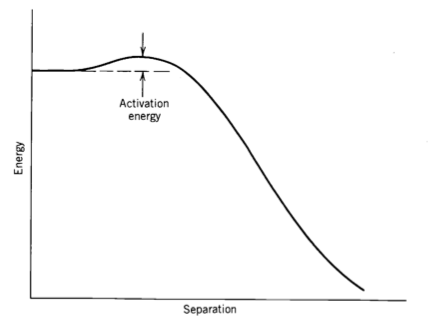
\includegraphics[scale=0.7]{smooth_fission_barrier.png}
 	\caption{The smooth fission barrier, illustrating the activation energy. Figure from K.S. Krane p.481 \cite{Krane1988}}
 	\label{fig:smooth_fission_barrier}
 \end{figure}

\noindent The energy released in fission is about the same as the activation energy needed to overcome the fission barrier. Those nuceli that have an energy release though fission that allows them to overcome most of the fission barrier, have a highter probability of tunnelling through the barrier \cite{Krane1988} (p.481). This is a known effect from quantum physics: the lower and thinner the potential barrier a particle must overcome, the larger the probability of tunnelling though the barrier. These nuclei that see a thin potential barrier are thus called the spontaneously fissioning nuclei. However, most of the nuceli are not able to overcome much fission barrier by themselves, and thus they see a thick and high potential barrier, and the probability of tunnelling is vanishing. They are therefore not unstable to spontaneous fission. This explains why the number of spontaneously fissioning nuclei are few, even though it is energetically possible for plenty of the heavier nuclei to fission.


  \begin{figure} [tbp]
	\centering
	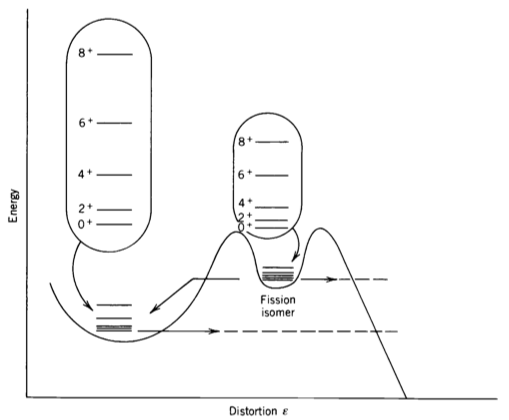
\includegraphics[scale=0.7]{double_humped_fission_barrier.png}
	\caption{The double humped fission barrier Figure from K.S. Krane p.496 \cite{Krane1988}}
	\label{fig:double_humped_fission_barrier}
\end{figure}

\par
\vspace{3mm}

\noindent This far  the fission barrier has only been described using the liquid drop model. However, the liquid drop model is not a complete description of the nuclei, and shell effects have a impact when studying the probability to fission. When including the effects of the single particle shell structure, the fission barrier is changed to a barrier with two humps, called the double-humped fission barrier \cite{Krane1988} (p.495). The double-humped fission barrier is shown in Figure \ref{fig:double_humped_fission_barrier}. Nuclei with energies below the fission barrier, but above the minima in the fission potential, sees two thinner barriers, compared to one thick barrier that the nuclei sees if it has energies below this well. They can tunnel through the first barrier, and then exist in an isomer state in the well, before either tunnelling through the second potential hump, or gamma-decay back to the ground state.  The tunnelling of two thin barriers is more probable than tunnelling through one thick barrier, so the double-humped fission barrier makes more nuclei unstable to spontaneous fission. The existence of the double-humped fission barrier was confirmed when fission isomers were discovered, which are isotopes highly unstable to spontaneous fission \cite{Krane1988} (p.495). 

\par
\vspace{3mm}

\noindent Even though states in the nucleus can have wave functions that have components in both the minimas of the double-humped fission barrier, the wave functions are usually are more prominent within one of the minimas \cite{Wagemans1991} (p.23). It is therefore common to separate them into class I and class II states, where class I states are states concentrated in the first well, while class II states are concentrated in the second well. 

For some elements, the double humped fission barrier is further extended to a humtiple-humped fission barrier \cite{Goriely2017}. The triple-humped fission barrier have been observed for actinides, and for some reaction channels \cite{PhysRevC.74.014608}. States that mainly exist within the third potential hump are, in accordance with the above definitions, referred to as class III states. 
 
\subsection{The role of fission in nucleosynthesis}
\label{fission_in_astro}
In the beginning of the new milennia, a comitee of physicists and astronomers presentet what they ment were the 11 greatest, unanswered questions withing physics \cite{Haseltine2002}. One of these was how heavy elements in the universe, raging from iron to uranium, was produced?

\par 
\vspace{3mm}
It has been known for some time that the light elements in the universe are produced through fusion of light elements into heavier elements. As seen from Figure \ref{fig:binding_energy_per_nucleon}, the average binding energy per nucleon increases up to about $A = 56$, and thus energy is released through fusion reactions. Iron, however, is the top of this curve. It is thus the bottom of the energy well, and energy can neither be released throug fission nor fusion. We know that elements up to uranium are produced somewhere in the universe, as we can observe them on Earth. This is why the comitee specified that the unanswered question is where in the universe the elements raging from iron to uranium are produced. 

\par
\vspace{3mm}

Physicist and astronomers are already underway of explaining the origin of plenty of the elements heavier than iron. Two processes often mentioned are the s-process and the r-process. Both are neutron capture processes. Iron can not fission nor fusion, but it can capture a neutron, and thus become unstable to $\beta$-decay. This way, as $\beta^{+}$-decay increases Z, new elements above iron are produced. The first of the two processes, the s-process, is the slow neutron-capture process, meaning that the frequency of neutron captures is low compared to the lifetimes of the nuclei created. It therefore only accounts for elements close to the valley of stability. The rapid neutron-capture process, however, consists of muntiple captures and decays, and can thus account for the production of far more unstable and heavier element than the s-process. Thus, the r-process needs a much higher neutron flux to occur, compared to the s-process. Through the s- and r-processes, and several more processes, one is beginning to see the outline of the isotope composition of the universe. Still, there is a long way to go before one of the great unanswered questions in physics can be ticked off the list.

\par 
\vspace{3mm}

As mentioned above, the r-process produces heavy, neutron-rich nuclei. These are often thought of to $\beta$-decay back to the valley of stability, but this is by far not the only possible reaction channel they can undergo. These nuclei can also undergo fission, and then produce several new, lighter nuclei.

\par 
\vspace{3mm}
Fission is though to may be the production reaction for light nuclei, in the interval A$\approx 110 - 160$. This is because the way new elements would be produced is as the fission fragments from heavy, neutron rich nucleus. If these fission fragments are still located in an area with high neutron flux, the fission fragments will continue to absorb neutrons, again becoming heavy nuclei, which can fission again. This process is known as fission recycling \cite{Goriely2017}. When the neutron flux decreases, the recyclin process will stop, leaving the fission fragments to decay towards stability. Fission in nucelosynthesis is not only neutron induced, it can also be spontaneous or $\beta$-delayed fission, and also $\gamma$-induced, the latter often referred to as photofission \cite{Goriely2017}. 

\par 
\vspace{3mm}

When determining if we have understood the nucleosynthesis, we rely on simultions of the procuction of the elements, comparing it to the element distrubution we can observe in the universe today.  The challenge when determining the fission's role in the synthesis of heavy elements, is that there are plenty of nuclear properties needed as input to these simulations, half-lives, reaction channel cross sections and fission barriers to mention some. Not only are these properties not always measured for all elements that can be produced in the laberatory, but one also need these properties for exotic nuclei, far from the valley of stability. Predictions must then be used for describing these exotic nuclei's properties, making the simulations of the fission's role in nucleosynthesis unreliable and heavily model dependent. 

\section{Method}

\subsection{TALYS}

TALYS is a computer code for computing reaction cross sections for nuclear reactions \cite{TALYSmanual}, and it is a handy tool for predicting outcomes of experiments before conducting them. TALYS can simulate light incident particles for a wide range of energies, hitting nuclei in the atomic mass region $12<A>339$ \cite{TALYSmanual}. The code will then provide the cross sections for different reactions to occur. The code is also highly customizable. It will provide a set of default values and models that can easily changed to study the impact of different models on the reaction cross sections.

\subsubsection{TALYS as a HF code}
TALYS is, as mentioned, a code for calculating reaction cross sections, and it has implemented several reaction models for different reactions. One of these models that are implemented, is the Hauser-Feshbach (HF) theory for compound nuclear reaction \cite{TALYSweb}. 
\par 
\vspace{3mm}

Hauser-Feshbach assumes the formation of a so-called compound nucleus when a reaction happens, which means the energy of the incoming particle is shared between all the nucleons in the nucleus. The compound nucleus, often excited, is thought to exist for a moment before decaying. The HF theory assumes that how this compound nuclei was formed is of no consequence. It claims there is no correlation between the incoming and the outgoing reaction channel \cite{Goriely2017}. The cross-section for a given reaction to happen is simply modelled like the cross section to form a given compound nucleus, multiplied with the cross section for this compoun nucleus to decay in a given way. 
\par 
\vspace{3mm}

There are some limitations to the HF theory. For one, it operates in the continuum region of excited levels \cite{Goriely2017}, and the calculations does therefore not include individual resonances. Furthermore, the model assumes the formation of a compound nucleus. This is not the case in all reactions, as the formation of a compound nucleus dominates at low energies and for heavy nuclei \cite{Goriely2017}. Hauser-Feshback theory is known to not be applicable to for example elastic scattering, where the incoming and outgoing reaction cross sections are the same  \cite{Goriely2017}.


\subsection{(n,$\gamma$) and (n,f) cross sections sensitivity to changes in the fission barrier of $\ce{^{240}Pu}$}


To model the impact of the uncertainty in the fission barrier of $\ce{^{241}Pu}$, and thus the impact of this uncertainty in the (n,f) and (n,$\gamma$) cross sections, the range of incoming neutron energies must first be chosen. My master experiment is the (d,p)-induced fission of $\ce{^{240}Pu}$, and it is used as the surrogate reaction of (n,f), assuming that the incoming reaction channel does not affect the reaction cross sections. I will thus calculate the cross sections for $\ce{^{240}Pu}$(n,f) with TALYS. The incoming deuteron energy used in the experiment will be $\approx$ 12 MeV, but the proton will carry some of this kinetic energy away from the nucleus. Thus we expect the neutron to carry up to 5 MeV to the nucleus, and therefore I will use neutron energies up to 5 MeV in this simulation. 
\par 
\vspace{3mm}

\noindent There are several choices of fission barrier models in TALYS. I have used the default one, which is an experimental fission barrier that contains data for fission barrier heights and shapes for actinides. \cite{TALYSmanual}. 

\par 
\vspace{3mm}


\noindent I first calculated the cross sections using the default fission barrier values in TALYS. I changed the theoretical fission barrier to so that the theoretical predictions reproduced experimental results. This value is further referred to as the theoretical value of the fission barrier. Thereafter, I varied the fission barrier within $\pm 1 \%$ of the theoretical value, and observed how the values for the fission and gamma cross section depended on the height of the fission barrier.

\section{Results}

\noindent I first calculated the  $\ce{^{240}Pu}$(n,f) and $\ce{^{240}Pu}$(n,$\gamma$) cross sections with the default values in TAYLYS, and compared them to experimental values. The results are shown in Figure \ref{fig:Default_TALYS_fission_xs_to_exp} and \ref{fig:Default_TALYS_gamma_xs_vs_exp}. 

  \begin{figure} [H]
	\centering
	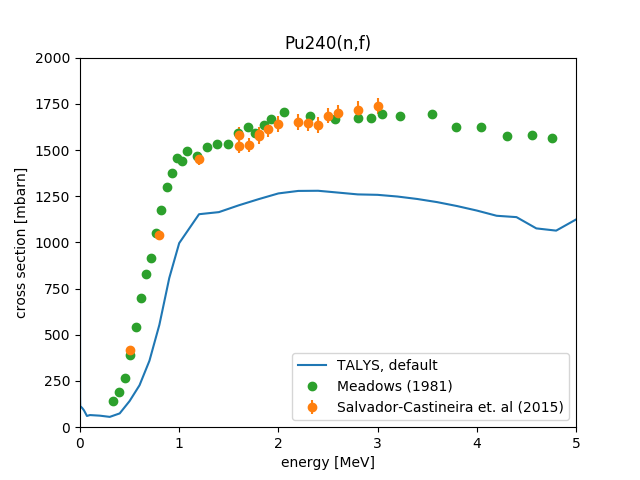
\includegraphics[scale=0.7]{Default_TALYS_fission_xs_to_exp.png}
	\caption{The default $\ce{^{240}Pu}$(n,f) cross section compared to experiments conducted by Salvador-Castinera et al. (2015) \cite{SALVADORCASTINEIRA2015177} and Meadows (1981) \cite{Meadows198}. The cross sections are plotted as a function of incoming neutron energy }
	\label{fig:Default_TALYS_fission_xs_to_exp}
\end{figure}

  \begin{figure} [H]
	\centering
	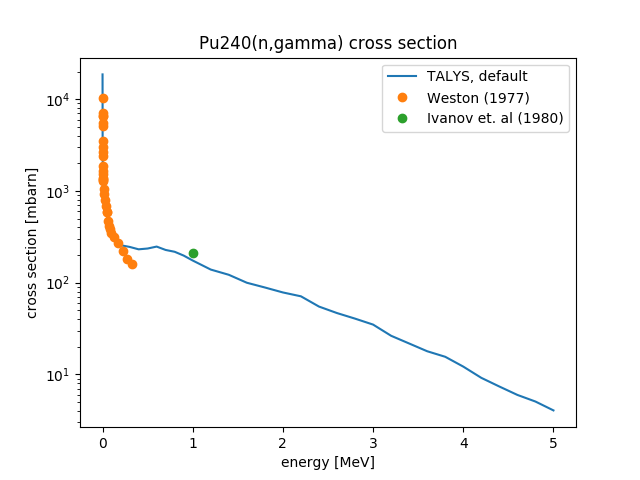
\includegraphics[scale=0.7]{Default_TALYS_gamma_xs_vs_exp.png}
	\caption{The default $\ce{^{240}Pu}$(n,f) cross section compared to experiments conducted by Salvador-Castinera et al. (2015) \cite{SALVADORCASTINEIRA2015177} and Meadows (1981) \cite{Meadows198}. The cross sections are plotted as a function of incoming neutron energy }
	\label{fig:Default_TALYS_gamma_xs_vs_exp}
\end{figure}

I changed the fission barrier such that the TALYS calculations mached the experimental results. The fitted fission barrier is shown in Figure \ref{fig:Modified_TALYS_gamma_xs_vs_exp}.

  \begin{figure} [H]
	\centering
	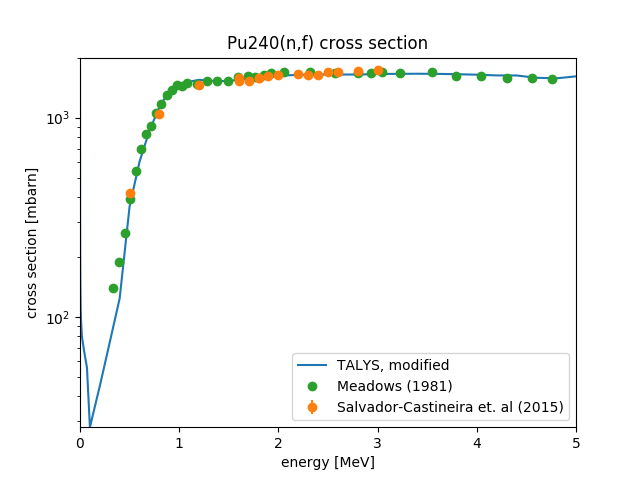
\includegraphics[scale=0.7]{Modified_TALYS_fission_xs_vs_exp.png}
	\caption{ $\ce{^{240}Pu}$(n,f) cross section with modified fission barrier, compared to experiments conducted by Salvador-Castinera et al. (2015) \cite{SALVADORCASTINEIRA2015177} and Meadows (1981) \cite{Meadows198}. The cross sections are plotted as a function of incoming neutron energy}
	\label{fig:Modified_TALYS_gamma_xs_vs_exp}
\end{figure}

I changed the fission barrier within $\pm 1 \%$, and plotted the fission and gamma cross sections. The results are shown in Figure \ref{fig:Fission_cross_section_varying_fission_barrier} and \ref{fig:Gamma_cross_section_varying_fission_barrier}. The scaling parameters used, first to fit the TALYS calculations to experimental results, and then to change the fission barrier within $\pm 1 \%$ is shown in Table \ref{tab:scalingparm_fission_barrier}. 

  \begin{figure} [H]
	\centering
	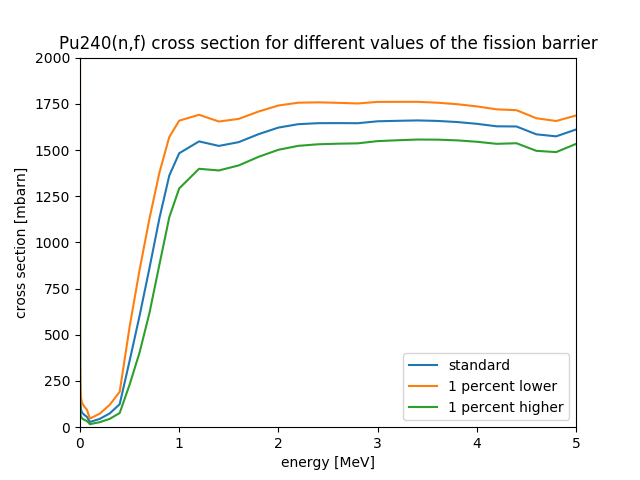
\includegraphics[scale=0.7]{Fission_cross_section_varying_fission_barrier.png}
	\caption{ $\ce{^{240}Pu}$(n,f) cross sections, when the fission barrier is changed within $\pm 1 \%$, plotted as a function of incoming neutron energy }
	\label{fig:Fission_cross_section_varying_fission_barrier}
\end{figure}

  \begin{figure} [H]
	\centering
	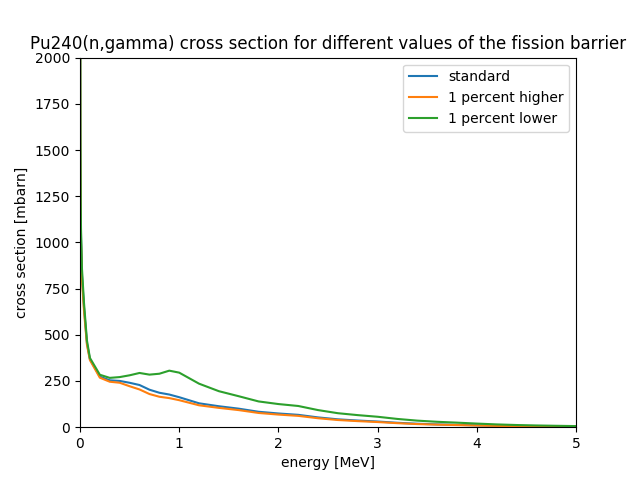
\includegraphics[scale=0.7]{Gamma_cross_section_varying_fission_barrier.png}
	\caption{ $\ce{^{240}Pu}$(n,$\gamma$) cross sections, when the fission barrier is changed within $\pm 1 \%$, plotted as a function of incoming neutron energy}
	\label{fig:Gamma_cross_section_varying_fission_barrier}
\end{figure}

\begin{table} [H]
	\centering
	\caption{Scaling parameters, used to fit the theory to experimental results, and thereafter to change the fission barrier within $\pm 1 \%$. As this is a double-humped fission barrier, there is one scaling parameter for each hump. The parameters are given as parts of the default sizes of fission barrier provided by TALYS}
	\begin{tabularx}{\textwidth}{XXX} \hline
		\label{tab:scalingparm_fission_barrier}
		Barrier & First hump scaling parameter & Second hump scaling parameter\\ \hline
		Theory to experiment & 0.975 & 0.900 \\
		$1 \% $ higher & 0.985  & 0.909  \\
		$1 \% $ lower & 0.965 & 0.891 \\ \hline
	\end{tabularx}
\end{table}

\section{Discussion}

As the reader can se from Figure \ref{fig:Default_TALYS_fission_xs_to_exp}, where the default TALYS settings for the neutron-induced fission of $\ce{^{240}Pu}$ is plotted against experimental results, there is a significant deviation between theory and experiment. There can be a number of reasons for this. As mentioned earlier, TALYS is highly customizable. For the fission barrier, there are several different models that can be used to model the fission barrier \cite{TALYSmanual}. This could be one of the reasons why the default calculation and the experiments didn't mach. However, it is hard to find a physical explanation to why there is a discrepancy, and I will not focus on finding this explanation in this report. 

\par 
\vspace{3mm}

 \noindent For my answers to be realistic when studying how the cross sections changes under a chage in the fission barrier, I first had to start with a fission barrier that reproduced the experimental results. I chose therefore to scale the default fission barrier. As described in section \ref{Theory}, for some nuclei the double-humped fission barrier is the best model for a fission barrier, and this is true for $\ce{^{241}Pu}$. I therefore scaled both the first and second hump with different scaling parameters until I found a good fit. This is not the best way to handle this challenge, as it does not explain why there is a difference.
 
 \par 
 \vspace{3mm}
 \noindent Thereafter, the fission parameter was scaled up and down within $\pm 1 \%$. As expected, the fission cross section was dependent on the height of the fission barrier, as seen in Figure \ref{fig:Fission_cross_section_varying_fission_barrier}. For lower incoming neutron energies, the cross sections show little deviation, but for the energy range $E_n \in [2,4]$ MeV, the fission cross sections show a deviation up to $\pm 100$ mb. This is a prominent difference. As talked over in section \ref{fission_in_astro}, if the fission barrier of $\ce{^{241}Pu}$ had this much uncertainties and the value was needed as an input parameter to a simulation, the result of the simulation would propably have high uncertainties. For $E_n > 4$ MeV, the deviation in fission cross sections seem to become smaller.
 
 \par 
 \vspace{3mm}
 \noindent In contrast to the fission cross section, the radiative neutron capture (n, $\gamma$)-cross sections seem not disturbed by the change in the fission barrier, as seen in Figure \ref{fig:Gamma_cross_section_varying_fission_barrier}. There is only a slight change in the region around $E_n = 1$MeV, where the cross section rises slightly for a higher fission barrier. This is as expected, as since the cross section for fission is lower, other reaction channels, as (n, $\gamma$), will be preferred. An explanation for why the (n,$\gamma$) cross section idoes not show more deviation for higher $E_n$, is that the cross section is already low in this region, because other reaction channels dominate. Rather than seeing a change in the (n,$\gamma$)-cross sections, one would expect to see a change in the channels that dominate for these energies. 


\section{Conclusion}
Based on the (somewhat very) crude calculations made in this report, it can be said that the fission cross section is highly sensitive to changes in the fission barrier, as was expected. This means that if there is an uncertainty in the fission barrier, simulations of cross sections might yield very different answers based on what value for the fission barrier is chosen. However, as mentioned, this report handles only very simple and shallow simulations, and can for example not explain why the default TALYS fission cross sections and the experimental ones deviate very much. The conclusion is thus that the fission cross section is sensitive to changes in the fission barrier, and for a better understanding of how sensitive, further deeper studies must be conducted. 

A question asked in the introduction was whether TALYS would be able to predict the fission cross sections in my master experiment. As I was unable to explain why the fission barrier in TALYS had to be scaled to experimental values before use, I am not eager to base my master thesis on results from this report. Again, further analysis would have to be conducted before there results can be counted as anything else than indications. 


\bibliographystyle{plain}
\bibliography{TALYS.bib} 






\end{document}
